\documentclass[12pt]{article}
\usepackage[paper=letterpaper,margin=2cm]{geometry}
\usepackage{amsmath}
\usepackage{amssymb}
\usepackage{amsfonts}
\usepackage{newtxtext, newtxmath}
\usepackage{enumitem}
\usepackage{titling}
\usepackage{svg}
\usepackage{xcolor}
\usepackage{listings}
\usepackage{float}
\usepackage{multicol}
\usepackage{nicefrac}
\usepackage{ragged2e}
\usepackage[autostyle]{csquotes}
\usepackage[colorlinks=true]{hyperref}

\MakeOuterQuote{"}
\setlength{\droptitle}{-6em}

\definecolor{codegreen}{rgb}{0,0.6,0}
\definecolor{codegray}{rgb}{0.5,0.5,0.5}
\definecolor{codepurple}{rgb}{0.58,0,0.82}
\definecolor{backcolour}{rgb}{0.95,0.95,0.92}

\lstdefinestyle{mystyle}{
    commentstyle=\color{codegreen},
    keywordstyle=\color{magenta},
    numberstyle=\tiny\color{codegray},
    stringstyle=\color{codepurple},
    basicstyle=\ttfamily\footnotesize,
    breakatwhitespace=false,
    breaklines=true,
    captionpos=b,
    keepspaces=true,
    numbers=left,
    numbersep=5pt,
    showspaces=false,
    showstringspaces=false,
    showtabs=false,
    tabsize=2
}

\lstset{
        style=mystyle,
        inputencoding=utf8,
        extendedchars=true,
}


\title{\large{Aprendizagem 2022}\vskip 0.2cm Homework III -- Group 019\vskip 0.2cm Diogo Gaspar 99207, Rafael Oliveira 99311}
\date{}
\begin{document}
\maketitle
\center\large{\vskip -2.5cm\textbf{Part I}: Pen and paper}
\begin{enumerate}[leftmargin=\labelsep]

  \item \textbf{Consider the basis function, $\phi_j(x) = x^j$, for performing a 3-order polynomial regression,
          $$
            \hat{z}(x, w) = \sum_{j=0}^3 w_j \phi_j(x) = w_0 + w_1 x + w_2 x^2 + w_3 x^3.
          $$
          Learn the Ridge regression ($l_2$ regularization) on the transformed data space
          using the closed-form solution with $\lambda = 2$.
        }

        We have in hands a \textbf{supervised learning} problem, with a given training
        dataset as shown below:

        \begin{table}[h]
          \centering
          \begin{tabular}{c|c|c}
                  & $y_1$ & $z$  \\ \hline
            $x_1$ & $0.8$ & $24$ \\
            $x_2$ & $1$   & $20$ \\
            $x_3$ & $1.2$ & $10$ \\
            $x_4$ & $1.4$ & $13$ \\
            $x_5$ & $1.6$ & $12$
          \end{tabular}
          \caption{Training dataset: $y_1$ as the input's (only) variable, $z$ as the target variable}
          \label{tab:training-dataset}
        \end{table}

        We can note that in the statement's estimation function, $\hat{z}(x, w)$, $x$ is a single-element vector
        (with its only entry being each sample's $y_1$ value). Therefore, it makes
        sense to "expand" the table above as follows, in order to have a broader
        representation of the values we'll end up using in the estimation function:

        \begin{table}[h]
          \centering
          \begin{tabular}{c|ccc|c}
                  & $y_1$ & $y_1^2$ & $y_1^3$ & $z$  \\ \hline
            $x_1$ & $0.8$ & $0.64$  & $0.512$ & $24$ \\
            $x_2$ & $1$   & $1$     & $1$     & $20$ \\
            $x_3$ & $1.2$ & $1.44$  & $1.728$ & $10$ \\
            $x_4$ & $1.4$ & $1.96$  & $2.744$ & $13$ \\
            $x_5$ & $1.6$ & $2.56$  & $4.096$ & $12$
          \end{tabular}
          \caption{Training dataset with additional information}
          \label{tab:expanded-training-dataset}
        \end{table}

        The equation below shows the closed-form solution for the Ridge regression
        problem, with $\lambda = 2$:

        \begin{equation*}
          % account for lambda, the bias term
          w = (\Phi^T \Phi + \lambda I)^{-1} \Phi^T z = (\Phi^T \Phi + 2 I)^{-1} \Phi^T z
        \end{equation*}

        Here, $\Phi$ is the result of applying the basis function to our training
        dataset's inputs, such that:

        \begin{equation*}
          \Phi = \begin{bmatrix}
            1      & \phi_1(x_1) & \phi_2(x_1) & \phi_3(x_1) \\
            1      & \phi_1(x_2) & \phi_2(x_2) & \phi_3(x_2) \\
            \vdots & \vdots      & \vdots      & \vdots      \\
            1      & \phi_1(x_5) & \phi_2(x_5) & \phi_3(x_5)
          \end{bmatrix} = \begin{bmatrix}
  1 & 0.8 & 0.64 & 0.512\\
  1 & 1 & 1 & 1\\
  1 & 1.2 & 1.44 & 1.728\\
  1 & 1.4 & 1.96 & 2.744\\
  1 & 1.6 & 2.56 & 4.096\\
\end{bmatrix}
        \end{equation*}

        We are now able to learn the given polynomial regression model, with $\lambda = 2$:
        $$
          \begin{aligned}
            (\Phi^T \Phi + \lambda I)^{-1}
             & = \left(
            \begin{bmatrix}
  1 & 0.8 & 0.64 & 0.512\\
  1 & 1 & 1 & 1\\
  1 & 1.2 & 1.44 & 1.728\\
  1 & 1.4 & 1.96 & 2.744\\
  1 & 1.6 & 2.56 & 4.096\\
\end{bmatrix}^T
            \begin{bmatrix}
  1 & 0.8 & 0.64 & 0.512\\
  1 & 1 & 1 & 1\\
  1 & 1.2 & 1.44 & 1.728\\
  1 & 1.4 & 1.96 & 2.744\\
  1 & 1.6 & 2.56 & 4.096\\
\end{bmatrix} +
            \begin{bmatrix}
  2 & 0 & 0 & 0\\
  0 & 2 & 0 & 0\\
  0 & 0 & 2 & 0\\
  0 & 0 & 0 & 2\\
\end{bmatrix}
            \right)^{-1}                        \\
             & = \begin{bmatrix}
  0.341688 & -0.121426 & -0.0749023 & -0.00932537\\
  -0.121426 & 0.389208 & -0.0966772 & -0.0744562\\
  -0.0749023 & -0.0966772 & 0.372578 & -0.17135\\
  -0.00932537 & -0.0744562 & -0.17135 & 0.179988\\
\end{bmatrix} \\
          \end{aligned}
        $$

        \begin{equation*}
          \Phi^T z = \begin{bmatrix}
  1 & 0.8 & 0.64 & 0.512\\
  1 & 1 & 1 & 1\\
  1 & 1.2 & 1.44 & 1.728\\
  1 & 1.4 & 1.96 & 2.744\\
  1 & 1.6 & 2.56 & 4.096\\
\end{bmatrix}^T
          \begin{bmatrix}
  24\\
  20\\
  10\\
  13\\
  12\\
\end{bmatrix} = \begin{bmatrix}
  79\\
  88.6\\
  105.96\\
  134.392\\
\end{bmatrix}
        \end{equation*}

        \begin{equation*}
          w = (\Phi^T \Phi + \lambda I)^{-1} \Phi^T z = \begin{bmatrix}
  7.04508\\
  4.64093\\
  1.96734\\
  -1.30088\\
\end{bmatrix}
        \end{equation*}

        Having learned the regression model, we can now use it to predict labels $z$
        for new samples!

        \pagebreak

  \item \textbf{Compute the training RMSE for the learnt regression model.}

        We know that the Root Mean Squared Error (RMSE) for a given regression model is
        defined as

        \begin{equation*}
          \text{RMSE} = \sqrt{\frac{1}{N} \sum_{i=1}^N (z_i - \hat{z}_i)^2},
        \end{equation*}

        where $N$ is the number of samples in the dataset, $z_i$ is the true label for
        the $i$-th sample, and $\hat{z}_i$ is the predicted label for the $i$-th sample.
        As stated in the previous question's statement, $\hat{z}$ is given by the matrix product
        $\Phi \cdot w$. We can, then, compute the RMSE for the training dataset as follows:

        \begin{equation*}
          \begin{aligned}
            \hat{z} = \Phi \cdot w & = \begin{bmatrix}
  1 & 0.8 & 0.64 & 0.512\\
  1 & 1 & 1 & 1\\
  1 & 1.2 & 1.44 & 1.728\\
  1 & 1.4 & 1.96 & 2.744\\
  1 & 1.6 & 2.56 & 4.096\\
\end{bmatrix} \cdot \begin{bmatrix}
  7.04508\\
  4.64093\\
  1.96734\\
  -1.30088\\
\end{bmatrix}
            = \begin{bmatrix}
  11.3509\\
  12.3525\\
  13.1992\\
  13.8287\\
  14.1785\\
\end{bmatrix}                                                                                 \\
            \text{RMSE}            & = \sqrt{\frac{1}{5} \sum_{i=1}^5 (z_i - \hat{z}_i)^2}                                    \\
                                   & = \sqrt{\frac{1}{5} \left( (24 - 11.35086463)^2 + \hdots + (12 - 14.17854143)^2 \right)} \\
                                   & = 6.84329
          \end{aligned}
        \end{equation*}

        \pagebreak

  \item \textbf{Consider a multi-layer perceptron characterized by one hidden layer with 2 nodes.
          Using the activation function $f(x) = e^{0.1x}$ on all units, all weights
          initialized as 1 (including biases), and the half squared error loss, perform
          one batch gradient descent update (with learning rate $\eta = 0.1$)
          for the first three observations (0.8), (1) and (1.2).
        }

        As a side-note, we'll be using the following notation in order to represent the resulting column matrix $X'$
        of the sum of all entries $X_{ji}$ in a given line $j$, for all lines of the original matrix $X$:

        $$
          \Sigma_X = X' = \begin{bmatrix}
            X_{11} + X_{12} + \hdots + X_{1n} \\
            X_{21} + X_{22} + \hdots + X_{2n} \\
            \vdots                            \\
            X_{m1} + X_{m2} + \hdots + X_{mn}
          \end{bmatrix}
        $$

        This notation will be particularly useful in the latter section of this
        question's answer.

        Our multi-layer perceptron, considering the parameters stated above, should only
        have one output-node, since we're considering a regression problem aiming to
        predict a single output variable.

        Each node in the hidden layer has an activation function $f(x) = e^{0.1x}$.
        Moreover, we know that the learning rule for the weights of each layer $l$
        is given by $\Delta w^{[l]} = - \eta \frac{\partial E}{\partial w^{[l]}}$ (with an analogous
        logic associated to biases), with $\eta = 0.1$ and $E$ being the half squared error loss:
        $E = \frac{1}{2} \sum_{i=1}^N (z_i - \hat{z}_i)^2$.

        A gradient descent update will require us to go through 3 phases: forward
        propagation, back propagation and updates (via gradient updates, updating
        biases and weights).

        Starting by the forward propagation, and considering $l$ as a given layer,
        we have (where $i$ matches the $i$-th sample):

        \begin{equation*}
          z_i^{[l]} = w^{[l]} x_i^{[l]} + b^{[l]}, \quad x_i^{[l]} = f\left(z_i^{[l]}\right)
        \end{equation*}

        We also know, from the question's statement, both the input nodes' values
        and weight/bias matrices (considering a column per sample for $x$):

        \begin{equation*}
          \begin{aligned}
            x^{[0]} = \begin{bmatrix}
  0.8 & 1 & 1.2\\
\end{bmatrix}
          \end{aligned}
        \end{equation*}
        \begin{equation*}
          \begin{aligned}
            w^{[1]} & = \begin{bmatrix}
  1\\
  1\\
\end{bmatrix}, \quad
            b^{[1]} & = \begin{bmatrix}
  1\\
  1\\
\end{bmatrix}, \quad
            w^{[2]} & = \begin{bmatrix}
  1 & 1\\
\end{bmatrix}, \quad
            b^{[2]} & = \begin{bmatrix}
  1\\
\end{bmatrix}
          \end{aligned}
        \end{equation*}

        \pagebreak

        Applying the afore-mentioned equations in succession will lead us to the following results
        (note that, just like with $x$, we'll also have one column per sample
        for $z^{[l]}$):


        \begin{equation*}
          \begin{aligned}
             & z^{[1]} = \begin{bmatrix}
  1.8 & 2 & 2.2\\
  1.8 & 2 & 2.2\\
\end{bmatrix} \quad
             & z^{[2]} = \begin{bmatrix}
  3.39443 & 3.44281 & 3.49215\\
\end{bmatrix}       \\
             & x^{[1]} = \begin{bmatrix}
  1.19722 & 1.2214 & 1.24608\\
  1.19722 & 1.2214 & 1.24608\\
\end{bmatrix} \quad
             & x^{[2]} = \begin{bmatrix}
  -1\\
  1\\
\end{bmatrix}
          \end{aligned}
        \end{equation*}

        We'll want, now, to propagate information backwards; for that, we'll need to use
        the chain rule, multiplying successive derivatives as we go backwards.
        With $L$ being the \textbf{last layer} - will be useful for reusing previously
        calculated $\delta$'s - we have the following equalities:

        \begin{equation*}
          \begin{aligned}
            \delta^{[L]}                        & = \textcolor{teal}{\frac{\partial E}{\partial x^{[L]}} \circ
            \frac{\partial x^{[L]}}{\partial z^{[L]}}}                                                                             \\
            \delta^{[l]}                        & =
            \frac{\partial z^{[l + 1]^T}}{\partial x^{[l]}} \cdot \delta^{[l + 1]} \circ \frac{\partial x^{[l]}}{\partial z^{[l]}} \\
            \frac{\partial E}{\partial w^{[l]}} & = \textcolor{teal}{\delta^{[l]}}
            \frac{\partial z^{[l]^T}}{\partial w^{[l]}}                                                                            \\
            \frac{\partial E}{\partial b^{[l]}} & = \textcolor{teal}{\delta^{[l]}}
            \frac{\partial z^{[l]^T}}{\partial b^{[l]}}
          \end{aligned}
        \end{equation*}

        Note that, this way, we'll be able to create a matrix $\delta^{[l]}$ for each
        layer $l$, where each column $i$ has the calculated $\delta_i^{[l]}$.
        We'll now be able to start propagating backwards (considering the following equalities,
        derived both in class and in the curricular unit's book):

        % derivative of the error loss

        \begin{equation*}
          \begin{aligned}
            \frac{\partial E}{\partial x_i^{[2]}} = \frac{\partial \frac{1}{2}\sum_{i=1}^N (z_i - x_i^{[2]})^2}{\partial x_i^{[2]}} = \sum_{i=1}^N (x_i^{[2]} - z_i), \quad
            \frac{\partial x_i^{[l]}}{\partial z_i^{[l]}} = \frac{\partial e^{0.1z_i^{[l]}}}{\partial z_i^{[l]}} = 0.1e^{0.1z_i^{[l]}}
          \end{aligned}
        \end{equation*}

        \begin{equation*}
          \begin{aligned}
            \frac{\partial z_i^{[l]}}{\partial x_i^{[l - 1]}} = w^{[l]}, \quad
            \frac{\partial z_i^{[l]}}{\partial b^{[l]}} = 1, \quad
            \frac{\partial z_i^{[l]}}{\partial w^{[l]}} = x_i^{[l - 1]}
          \end{aligned}
        \end{equation*}

        \begin{equation*}
          \begin{aligned}
            \textcolor{purple}{\delta^{[2]}} & = \left[\sum_{i=1}^N(x_i^{[2]} - z_i)\right] \circ 0.1e^{0.1z^{[2]}}            \\
                                             & = \begin{bmatrix}
  -22.5958 & -18.589 & -8.58205\\
\end{bmatrix} \circ \begin{bmatrix}
  0.140417 & 0.141097 & 0.141795\\
\end{bmatrix} \\
                                             & = \begin{bmatrix}
  -3.17283 & -2.62286 & -1.2169\\
\end{bmatrix}
          \end{aligned}
        \end{equation*}

        \begin{equation*}
          \begin{aligned}
            \textcolor{purple}{\delta^{[1]}} & = \frac{\partial z^{[2]^T}}{\partial x^{[1]}} \cdot \delta^{[2]} \circ \frac{\partial x^{[1]}}{\partial z^{[1]}} \\
                                             & = \begin{bmatrix}
  -3.17283 & -2.62286 & -1.2169\\
  -3.17283 & -2.62286 & -1.2169\\
\end{bmatrix} \circ \begin{bmatrix}
  0.119722 & 0.12214 & 0.124608\\
  0.119722 & 0.12214 & 0.124608\\
\end{bmatrix}                           \\
                                             & = \begin{bmatrix}
  -0.379857 & -0.320357 & -0.151634\\
  -0.379857 & -0.320357 & -0.151634\\
\end{bmatrix}
          \end{aligned}
        \end{equation*}

        In the last phase, we'll be updating our model: after computing the gradients,
        we'll be able to update weights and biases!

        Starting with weight matrices:

        \begin{equation*}
          \frac{\partial E}{\partial w^{[1]}} = \textcolor{purple}{\delta^{[1]}} \cdot
          \frac{\partial z^{[1]^T}}{\partial w^{[1]}}
          = \textcolor{purple}{\delta^{[1]}} \cdot x^{[0]^T}
          = \begin{bmatrix}
  -0.806204\\
  -0.806204\\
\end{bmatrix}
        \end{equation*}

        \begin{equation*}
          \frac{\partial E}{\partial w^{[2]}}
          = \textcolor{purple}{\delta^{[2]}}
          \cdot x^{[1]^T}
          = \begin{bmatrix}
  -8.51849 & -8.51849\\
\end{bmatrix}
        \end{equation*}

        \begin{equation*}
          \begin{aligned}
            w^{[1]} = w^{[1]} - \eta \cdot \frac{\partial E}{\partial w^{[1]}}
             & = \begin{bmatrix}
  1\\
  1\\
\end{bmatrix} - 0.1 \cdot \begin{bmatrix}
  -0.806204\\
  -0.806204\\
\end{bmatrix}
            = \begin{bmatrix}
  1.08062\\
  1.08062\\
\end{bmatrix}
          \end{aligned}
        \end{equation*}

        \begin{equation*}
          \begin{aligned}
            w^{[2]} = w^{[2]} - \eta \cdot \frac{\partial E}{\partial w^{[2]}}
             & = \begin{bmatrix}
  1 & 1\\
\end{bmatrix} - 0.1 \cdot \begin{bmatrix}
  -8.51849 & -8.51849\\
\end{bmatrix} \\
             & = \begin{bmatrix}
  1.85185 & 1.85185\\
\end{bmatrix}
          \end{aligned}
        \end{equation*}

        After updating weights, we'll update biases:

        \begin{equation*}
          \frac{\partial E}{\partial b^{[1]}} = \Sigma_{\textcolor{purple}{\delta^{[1]}}} \cdot
          \frac{\partial z^{[1]^T}}{\partial b^{[1]}}
          = \Sigma_{\textcolor{purple}{\delta^{[1]}}} \cdot 1
          = \Sigma_{\textcolor{purple}{\delta^{[1]}}}
          = \begin{bmatrix}
  -0.379857 & -0.320357 & -0.151634\\
  -0.379857 & -0.320357 & -0.151634\\
\end{bmatrix}
        \end{equation*}

        \begin{equation*}
          \frac{\partial E}{\partial b^{[2]}} = \Sigma_{\textcolor{purple}{\delta^{[2]}}} \cdot
          \frac{\partial z^{[2]^T}}{\partial b^{[2]}}
          = \Sigma_{\textcolor{purple}{\delta^{[2]}}} \cdot 1
          = \Sigma_{\textcolor{purple}{\delta^{[2]}}}
          = \begin{bmatrix}
  -7.01259\\
\end{bmatrix}
        \end{equation*}

        \begin{equation*}
          \begin{aligned}
            b^{[1]} = b^{[1]} - \eta \cdot \frac{\partial E}{\partial b^{[1]}}
             & = \begin{bmatrix}
  1\\
  1\\
\end{bmatrix} - 0.1 \begin{bmatrix}
  -0.379857 & -0.320357 & -0.151634\\
  -0.379857 & -0.320357 & -0.151634\\
\end{bmatrix} \\
             & = \begin{bmatrix}
  1.08518\\
  1.08518\\
\end{bmatrix}
          \end{aligned}
        \end{equation*}

        \begin{equation*}
          \begin{aligned}
            b^{[2]} = b^{[2]} - \eta \cdot \frac{\partial E}{\partial b^{[2]}}
             & = \begin{bmatrix}
  1\\
\end{bmatrix} - 0.1 \cdot \begin{bmatrix}
  -7.01259\\
\end{bmatrix} \\
             & = \begin{bmatrix}
  1.70126\\
\end{bmatrix}
          \end{aligned}
        \end{equation*}

\end{enumerate}

\pagebreak

\center\large{\textbf{Part II}: Programming and critical analysis}

\begin{justify}
  The code utilized to answer the following questions is available in this
  report's appendix.
\end{justify}

\begin{enumerate}[leftmargin=\labelsep,resume]
  \item \textbf{Compute the MAE of the three regressors: linear regression, $MLP_1$ and $MLP_2$.}

        We opted to utilize \texttt{sklearn}'s \texttt{mean\_absolute\_error} function to compute the MAE of the three regressors.
        The regressors were created as shown in the appendix (using \texttt{Ridge} and
        \texttt{MLPRegressor} with the respective parameters).

        We gathered the following results:

        \begin{table}[h]
          \centering
          \begin{tabular}{l|l}
            Regressor                 & MAE       \\ \hline
            Linear Regression (Ridge) & $0.16283$ \\
            $MLP_1$                   & $0.06804$ \\
            $MLP_2$                   & $0.09781$
          \end{tabular}
          \caption{Gathered Mean Absolute Errors for each specified regressor}
          \label{tab:mean-absolute-errors}
        \end{table}

  \item \textbf{Plot the residues (in absolute value) using two visualizations: boxplots and histograms.}

        Each regressor's residues, calculated as the absolute difference between
        the predicted and actual values, were plotted using both boxplots and histograms
        (using, respectively, \texttt{seaborn}'s \texttt{boxplot} and \texttt{histplot} functions),
        as shown in this report's appendix (figure after the code).

  \item \textbf{How many iterations were required for $MLP_1$ and $MLP_2$ to converge?}

        Calling the \texttt{print\_regressor} method for each regressor shows us
        not only the MAE, but also the number of iterations required for each of
        the MLP regressors to converge. In this case, the number of iterations
        required for $MLP_1$ ($MLP$ with early stopping) to converge was 452,
        while $MLP_2$ ($MLP$ \textit{without} early stopping) required only 77.

  \item \textbf{What can be motivating the unexpected differences on the number of iterations?
          Hypothesize one reason underlying the observed performance differences between the MLPs.}

        As has been noted in the previous question's answer, $MLP_1$ takes many more
        iterations to converge than $MLP_2$ - almost six times as many. It's probably
        worth emphasizing that the number of iterations in a batch gradient descent
        algorithm matches the number of epochs ran - the amount of times the algorithm goes
        through the entire dataset.

        With \texttt{MLPRegressor}'s early stopping implementation, the training stops
        after a given number of epochs have passed without the validation score
        improving by at least a given tolerance (in order to avoid overfitting).
        The validation set, with \texttt{MLPRegressor}'s \texttt{shuffle} parameter
        set by default to True, may contain samples from both the training and test sets:
        with differing training sets (which forcefully seems like the case here),
        the training process may converge at a different amount of epochs; it's
        also likely that a training set with a lesser amount of samples may
        take more epochs to converge, as the algorithm will have to go through
        the entire dataset more times to reach the "same amount of samples seen"
        in order to better fit the data.

        The \textbf{different number of iterations} could, then, be associated
        with the differing training sets used to train each regressor, plus the
        fact that $MLP_1$ stops the validation phase tells it do so, while $MLP_2$
        strictly looks at convergence regarding training data.

        Regarding performance, $MLP_1$ seems to perform better than $MLP_2$,
        with a lower (and thus better) MAE, as stated in question 4.'s answer.
        Although both regressors end up converging in training, $MLP_1$ has
        the advantage of stopping right where the validation score starts to
        stagnate/decrease: this means that the regressor ends up not overfitting
        the data, as it would if it kept training for more epochs until reaching
        "regular" convergence, like $MLP_2$ (which appears to be a bit more overfitted,
        in comparison to $MLP_1$).


\end{enumerate}

\pagebreak

\large{\textbf{Appendix}\vskip 0.3cm}

\lstinputlisting[language=Python]{code.py}

\begin{figure}[H]
  \centering
  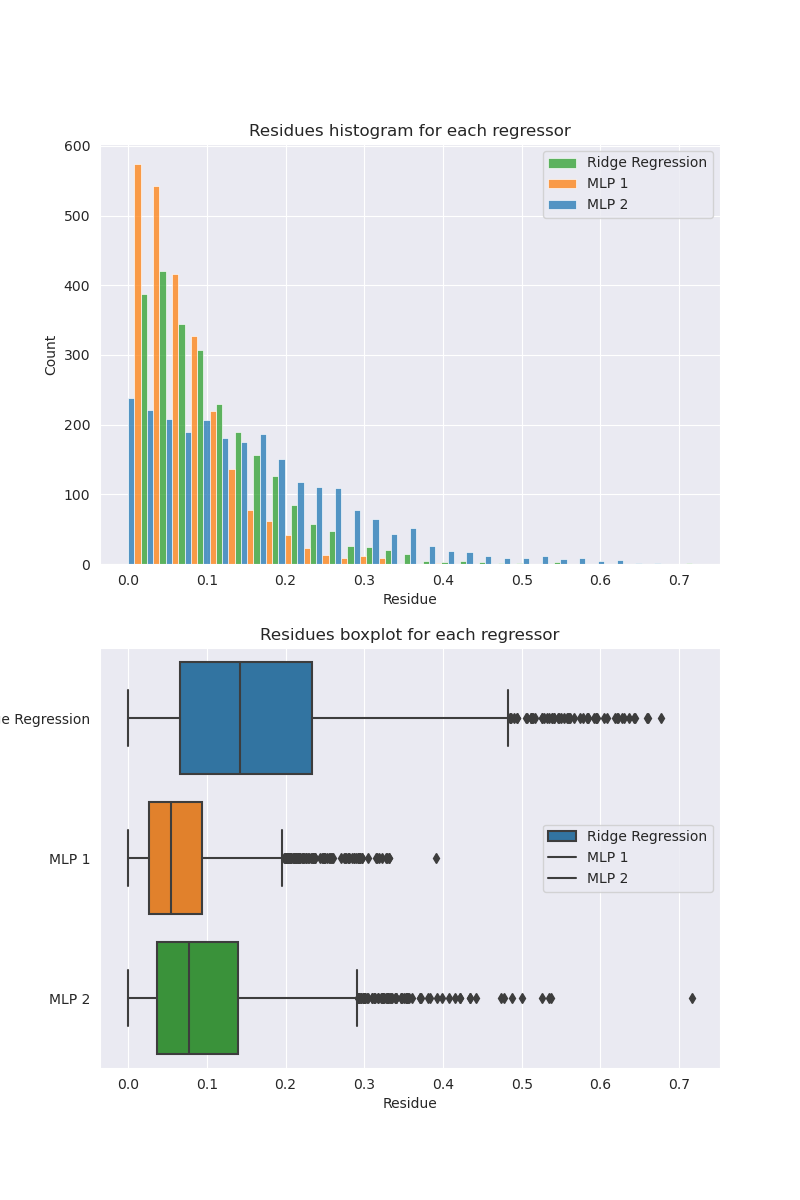
\includegraphics[width=0.8\textwidth]{../assets/residues.png}
  \caption{Ridge regression's residue plotting}
  \label{fig:residue-plotting}
\end{figure}

\end{document}
